\documentclass{standalone}
\usepackage[utf8]{inputenc}
\usepackage[T1]{fontenc}
\usepackage{graphicx}
\usepackage{amsmath}
\usepackage[american,siunitx]{circuitikz}
\usetikzlibrary{arrows,shapes,calc,positioning}

    
\begin{document}
  \begin{tikzpicture}[node distance=22mm, block/.style={rectangle, draw, minimum height=14mm, inner sep=2pt}, sumnode/.style={circle, draw, inner sep=4pt}]

    \node[block] (plant) {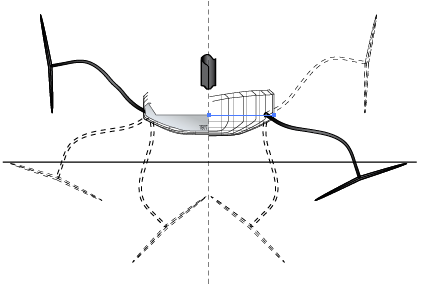
\includegraphics[height=26mm]{AC75-sketch.png}};
    \node[block, left of=plant, node distance=60mm] (actuator) {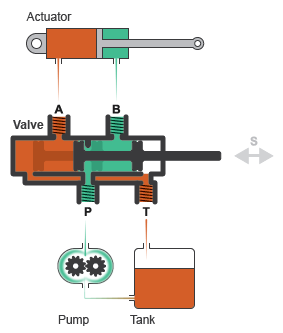
\includegraphics[height=40mm]{hydraulics.png}};
    \node[block, left of=actuator, node distance=46mm, align=center] (controller) {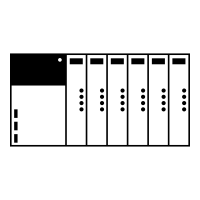
\includegraphics[width=16mm]{plc.png}\\Controlador};
    \node[block, right of=plant, node distance=70mm] (boat) {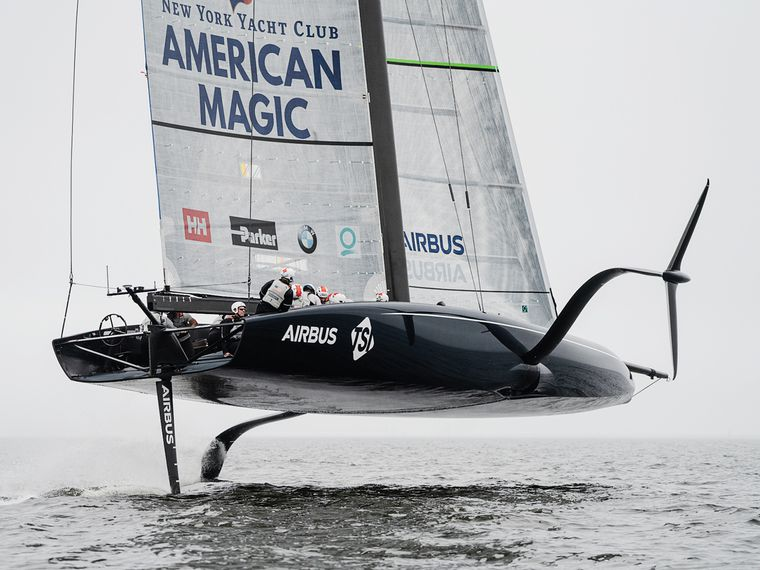
\includegraphics[height=40mm]{ac75.jpeg}};
    \node[coordinate, left of=controller, node distance=30mm] (input) {};
    \node[coordinate, right of=boat, node distance=48mm] (output) {};
    \node[coordinate, above of=plant, node distance=20mm] (disturbance) {};
    \node[coordinate, above of=boat, node distance=30mm] (disturbance2) {};
    \node[block, below of=plant, node distance=40mm] (sensor) {Sensor};
    \node[block, below of=boat, node distance=60mm] (sensor2) {Sensor};

    \draw[->] (input) -- node[above, pos=0.3, align=left] {posición\\deseada} (controller);
    \draw[->] (controller) -- node[above, align=left] {mueve\\ valvula} (actuator);
    \draw[->] (actuator) -- node[above] {fuerza} (plant);
    \draw[->] (plant) -- node[coordinate] (meas) {}  node[above,] {posición} (boat);
    \draw[->] (boat) -- node[coordinate] (meas2) {}  node[above, near end] {yacht state} (output);
    \draw[->] (disturbance) -- node[right, pos=0.2] {perturbación} (plant);
    \draw[->] (disturbance2) -- node[right, pos=0.2] {perturbación} (boat);
    \draw[->] (meas) |- (sensor) -| node[right, pos=0.9] {} (controller);
    \draw[->] (meas2) |- (sensor2) -| node[right, pos=0.9] {} (controller.south west);

    \node[red] at (2,-6) {\Huge $\times$};
  \end{tikzpicture}


\end{document}
